\documentclass{article}
\usepackage[utf8]{inputenc}
\usepackage{amsmath}
\usepackage{listings}
\usepackage{geometry}
\usepackage{graphicx}
\usepackage{appendix}
\usepackage{subfig}
\usepackage{gensymb}
\usepackage{cancel}
\usepackage{physics}
\usepackage[colorlinks=true]{hyperref}
\usepackage{xcolor}
\definecolor{codegreen}{rgb}{0,0.6,0}
\definecolor{codegray}{rgb}{0.5,0.5,0.5}
\definecolor{codepurple}{rgb}{0.58,0,0.82}
\definecolor{backcolour}{rgb}{0.95,0.95,0.92}
\lstdefinestyle{mystyle}{
    backgroundcolor=\color{backcolour},   
    commentstyle=\color{codegreen},
    keywordstyle=\color{magenta},
    numberstyle=\tiny\color{codegray},
    stringstyle=\color{codepurple},
    basicstyle=\ttfamily\footnotesize,
    breakatwhitespace=false,         
    breaklines=true,                 
    captionpos=b,                    
    keepspaces=true,                 
    numbers=left,                    
    numbersep=5pt,                  
    showspaces=false,                
    showstringspaces=false,
    showtabs=false,                  
    tabsize=2
}

\lstset{style=mystyle}

\title{%
Project 2 - Studying Quantum Mechanical Systems \\
with Restricted Boltzmann Machines \\
\large FYS4411 at University of Oslo}
\author{Simen Løken}
\date{June 2023}
\footskip = 90pt
\topmargin = -40pt

\begin{document}
\nocite{*}
\maketitle
{
  \hypersetup{linkcolor=black}
  \tableofcontents
}
\section{Abstract}
In this project, we will examine the how we can estimate the wavefunction of a quantum mechanical system using a Restricted Boltzmann Machine. We find that it can sufficiently model a system of two fermions with two degrees of freedom, without interaction, with very good energy estimates that are very close in value to the nominal $2.0 a.u.$ for such a system. We then extend the system to also include the interactive energy between the fermions, with somewhat lackluster results. Lastly, we quickly examine how a Restricted Boltzmann Machine could be replaced with an equivalent deep network, and see what kind of results it can yield.
\section{Introduction}
When working with quantum mechanics, traditionally we use wavefunctions to the describe and model the quantum states of the system. This is fine when working with small systems, but as the size and computational magnitude of the system increases, the resources required to represent and work with wavefunctions increases exponentially. This in turn makes it harder to study, explore and analyze quantum mechanical systems.
\newline
But all is not lost - in recent years the field of machine learning has seen significant advancement in terms of both deep learning and neural networks. One such method, and the method we're going to be studying today, is the Restricted Boltzmann Machine (RBM). It turns out RBMs provide a compact and efficient representation of quantum wavefunctions. The efficiency, expressive power and learning capabilities make them the an ideal choice when studying quantum mechanical systems
\newline In this project, we will therefore examine a simple quantum mechanical system of limited complexity, and use an RBM to model the appropriate wavefunction to see if we can approach the known analytical solutions to the energies of such a system, for both an uninteractive and a interactive case, respectively. Lastly, we will try to see if we can replace the RBM with a deep network to see if it also can estimate the wavefunction of the system. \newpage
\section{Theory and Method}
\subsection{The System}
In this project we will be studying a two-particle system of fermions. The fermions will be limited to two-dimensional movement. We will study the system both in terms of an interacting and a non-interacting case. That is to say, when measuring the energy of the system we will be, we will look at both purely the kinetic and potential energy of the fermions, and also at the interacting energy between the two particles.
\subsubsection{The non-interacting case}
Firstly, we will study the non-interacting case, simply because it is much simpler than than its interacting counterpart and also because such a system has a known energy. The energy of such a system can be expressed in atomic units (a.u.) by:
\begin{equation} \label{enrgy}
    E = N \cdot D
\end{equation}
where $N$ is the number of particles in the system and $D$ is the degrees of freedom of the particles (in this case 1, 2 or 3 for 1D, 2D and 3D respectively). Additionally, the system is modeled by a Hamiltonian:
\begin{equation}
    \hat H_0 = \sum_{i=1}^N \left( - \frac{1}{2}\nabla_i^2 + \frac{1}{2}\omega^2 r_i^2 \right)
\end{equation}
For the sake of simplicity, we let all natural units be 1, and set $\omega=1$. This will allow us to work with atomic units, which let's us easily compare with the known analytical energy given by Eq. [\ref{enrgy}]. 
\subsubsection{The interacting case}
Now for the more interesting case. We alluded to earlier that we would only be examining two fermions with two degrees of freedom. There is a reason for this, as the analytical energy value of such a system is known to be 3 a.u.. This in turn makes it easier for us to tune our model and test if it can accurately numerically predict the energy of an interacting case of two fermions. \newline
As for the Hamiltonian from above, given the interaction between the two particles, it gets an additional term:
\begin{equation} \label{H1}
    \hat H_1 = \sum_{i<j} \frac{1}{r_{ij}}
\end{equation}
such that the full Hamiltonian becomes:
\begin{equation} \label{ham}
    \hat H = \hat H_0 - \hat H_1 = \sum_{i=1}^N \left( - \frac{1}{2}\nabla_i^2 + \frac{1}{2}\omega^2 r_i^2 \right) + \sum_{i<j} \frac{1}{r_{ij}}
\end{equation}
The energy of such a system is described as:
\begin{equation} \label{locEn}
    E_L = \frac{1}{\Psi} \hat H \Psi
\end{equation}
where $\Psi$ is the wavefunction represented by the RBM. A full derviation and of this expression of energy can be found at Appendix \ref{AppEn}.
\subsection{Restricted Boltzmann Machines}
We're going to be working with a Gaussian-binary RBM instead of the original binary-binary RBM in the project. The RBM is a generative neural network model that has many use cases. In this case, we're going to use it to simulate the wavefunction of a quantum mechanical system. An RBM consists of a visible layer and a hidden layer. The visible layer represents the visible quantum states, whilst the hidden layer represents underlying connections. \newline
In our case, we let the visible layers represent the quantum states of the system and the hidden states the underlying quantum mechanical properties of the system. We can then model a joint probability distribution between the visible and hidden states to model the complexity of the wavefunction.
\newline
The joint probability distrubtion is given as:
\begin{equation}
    F_{rbm}(v,h) = \frac{1}{Z}) e^{-\frac{1}{T_0}E(v,h)}
\end{equation}
where $Z$ is defined as:
\begin{equation*}
    Z = \iint e^{-\frac{1}{T_0} E(v,h)}
\end{equation*}
Mathematically, we may define the energy of the RBM as:
\begin{equation}
    E(v, h) = \sum_i \frac{(v_i - b_{vi})^2}{2\sigma_i^2} - \sum_j b_{hj} h_j - \sum_{i,j} \frac{v_i w_{ij}h_j}{\sigma_i^2}
\end{equation}
\subsubsection{Contrastive Divergence}
When training RBMs, one of the most common methods is that of Contrastive Divergence (CD). The CD method approximates the gradient of the log-likelihood function by doing a series of Monte Carlo cycles, starting from the initial visible state and updating the visible and hidden states with each iteration. CD estimates the gradient by using a "phantom" particle from the model distribution and after a few sampling steps, subtracting the expectation given the current model distribution from the expectation of the "phantom" particle. We then use this approximation to update the RBM parameters.
\newline
The algorithm looks like this:
\begin{enumerate}
\item Sample the hidden states given the visible input using a sampling method.
\item Compute the positive gradient by taking the dot product between the transpose of the visible input and the sampled hidden states.
\item Perform sampling for a specified number of chains starting from the visible input.
\item Compute the negative gradient by taking the dot product between the transpose of the final chain state and the sampled hidden states.
\item Update the weights, visible biases, and hidden biases using the computed positive and negative gradients.
\item Repeat steps 1-5 until convergence or a predefined stopping criterion is met.
\end{enumerate}
This method is very effective in training an RBM, but there is an extension of this method that is even better.
\newline
The Persistent Contrastive Divergence (PCD) is an extension of CD. In PCD, instead of initializing a Markov Chain for each iteration, we instead maintain a persistent chain throughout the entire training process. The persistent chain is updated after each iteration using the "phantom" particle.
\begin{enumerate}
\item Sample the hidden states given the visible input using a sampling method.
\item Compute the positive gradient by taking the dot product between the transpose of the visible input and the sampled hidden states.
\item Perform sampling for a specified number of chains starting from the visible input.
\item Compute the negative gradient by taking the dot product between the transpose of the final chain state and the sampled hidden states.
\item Update the weights, visible biases, and hidden biases using the computed positive and negative gradients.
\item Sample the hidden states given the persistent chain using sampling.
\item Generate a visible state by sampling from the hidden units of the persistent chain, and then sample the hidden units based on this visible state.
\item Update the weights, visible biases, and hidden biases using the sampled persistent chain.
\item Repeat steps 1-8 until convergence or a predefined stopping criterion is met.
\end{enumerate}
The PCD, naturally, as an extension of CD, is better and faster than its unmodified counterpart. 
\newpage
\subsubsection{Gradient Descent}
Another very common method of training is the gradient descent method. Again we update the parameters of the RBM with each iteration, aiming to minimize a cost function. The cost function depends on the hidden biases $b_h$ and the visible biases $b_v$, together with the weights $w$
\newline
We aim to find the optimal values for the biases and weights that minimize the cost function like thus:
\begin{enumerate}
\item Sample the hidden states given the visible input using a sampling method.
\item Compute the positive gradient by taking the dot product between the transpose of the visible input and the sampled hidden states.
\item Sample the visible and hidden states again for reconstruction by starting from the visible input.
\item Generate a reconstructed visible state by sampling from the hidden units, and then sample the hidden units based on this reconstructed visible state.
\item Compute the negative gradient by taking the dot product between the transpose of the reconstructed visible state and the sampled hidden states.
\item Update the weights, visible biases, and hidden biases using the computed positive and negative gradients.
\item Repeat steps 1-6 until convergence or a predefined stopping criterion is met.
\end{enumerate}
\subsection{Sampling methods}
\subsubsection{Metropolis sampling}
When we say metropolis sampling, we refer to the Metropolis-Hastings algorithm, a Markov chain Monte Carlo method. The algorithm generates a sequence of samples from a target probability distribution. We construct a Markov chain [\ref{AppMa}] whose distribution is the target distribution. For each step in the chain, a sample is generated and then accepted or rejected based on the acceptance probability. The acceptance probability is chosen by the target distribution ratio at the generated and current state, respectively, along with a new proposed distribution.
\newline
In context of an RBM, we use metropolis sampling to sample from the RBMs learned distribution. We assign initial values values to the visible units, and for each iteration we we construct a Markov chain by updating the visible units given the current state. For a sufficient number of iterations, the samples will then approximate the true distribution of the wavefunction. This allows us to better model quantum mechanical systems, and allows the RBM to better model complex correlations and dependencies between the visible and hidden units
\newpage
\subsubsection{Importance sampling}
Importance sampling, as opposed to directly sampling from the target distribution, instead sample from an easier to sample distribution. We attempt to choose a distribution that is similar to the target distribution in areas of high importance (hence the name). This in turn often makes Importance sampling a better alternative to the perhaps more brute-force method of Metropolis sampling. In the case of Importance sampling, the very nature of it ensures that the proposed distribution is tailored to closely match the important regions of the target distribution. This leads to low(er) variance in the estimated numerical results.
\section{Results}
Let us first examine the non-interacting case with Metropolis sampling for all three training methods, CD, PCD and GD:
\begin{figure}[htbp]
  \centering
  \begin{minipage}[b]{0.3\textwidth}
    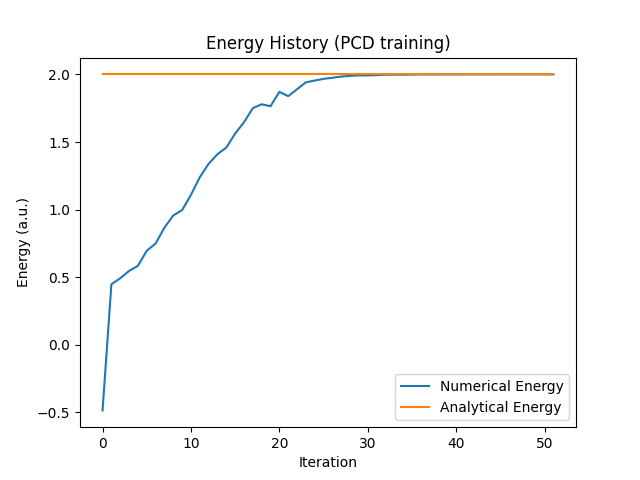
\includegraphics[width=\textwidth,height=0.6\textheight,keepaspectratio]{metroPCDnoInteract.png}
    \caption{Energy convergence per iteration for Persistent Contrastive Divergence}
    \label{fig:figure1a}
  \end{minipage}
  \hfill
  \begin{minipage}[b]{0.3\textwidth}
    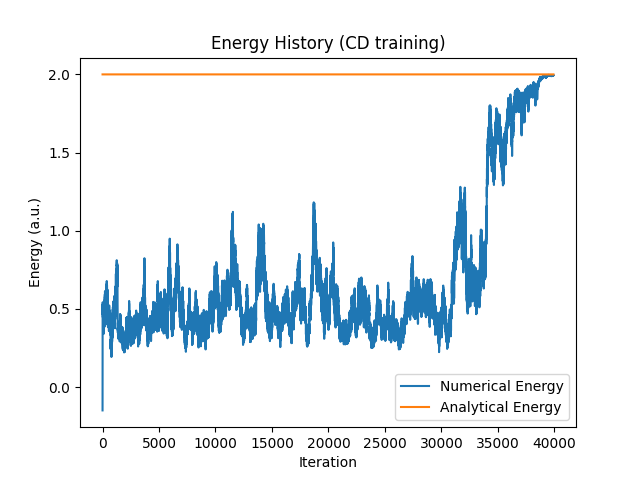
\includegraphics[width=\textwidth,height=0.6\textheight,keepaspectratio]{metroCDnoInteract.png}
    \caption{Energy convergence per iteration for Contrastive Divergence}
    \label{fig:figure1b}
  \end{minipage}
  \hfill
  \begin{minipage}[b]{0.3\textwidth}
    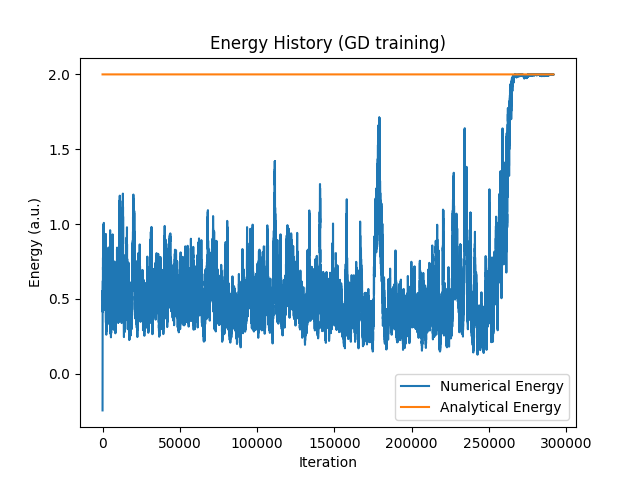
\includegraphics[width=\textwidth,height=0.6\textheight,keepaspectratio]{metroGDnoInteract.png}
    \caption{Energy convergence per iteration for Gradient Descent}
    \label{fig:figure1c}
  \end{minipage}
  \caption*{Here we see how the energy converges over iterations for Metropolis sampling\newline
    $\eta = 0.005$, $h.u. = 16$}
\end{figure}
\newline
We see here that PCD performs by far the best, converging much earlier. We should note that this isn't a one-time occurrence. PCD generally needs less than 100 iterations to converge at an energy value. Of course, this depends on other factors and variables, but it is generally much, much faster. In terms of iterations, GD performs worse than CD, but it is worth mentioning that an iteration of GD is much faster than a CD iteration, so much so that GD is actually, despite the iterations, two times faster than that of CD. \newline
On the next page we will examine a table of results and errors for a set of initial variables:
\newpage
\begin{table}[ht!]
    \centering
    \begin{tabular}{c|c|c}
     Type& Result [a.u.]& Error [a.u.]&
     \hline
     PCD&  2.00& 2.16\times10^{-7}\\
     CD& 2.00& 5.57\times10^{-5}\\
     GD& 2.00& 4.69\times10^{-5}
    \end{tabular}
    \caption{The results given metropolis sampling and a blocking analysis with the following variables:
    \newline MC Cycles: 4992, Hidden Units: 16, Visible Units: 4, $\eta$: 0.005, Sweeps: 100, Chain length: 100
    }
    \label{tab:metro}
\end{table}
\newline
We see here that all methods can accurately predict the numerical energy value of a 2 dimensional system with 2 fermions with varying degrees of error. PCD performs the best whilst being much faster than the other algorithms.
\begin{figure}[htbp]
  \centering
  \begin{minipage}[b]{0.3\textwidth}
    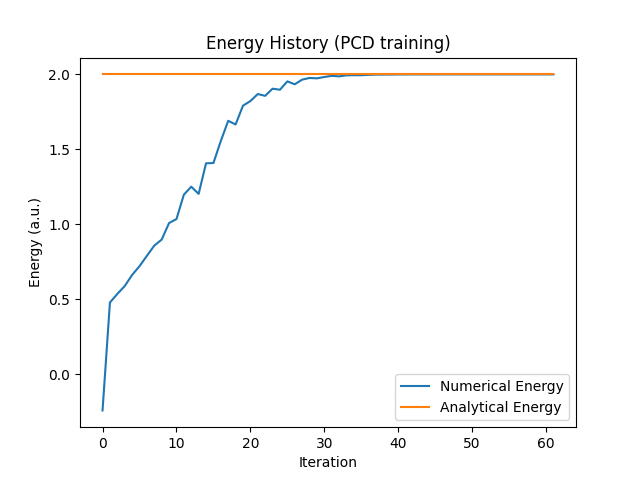
\includegraphics[width=\textwidth,height=0.6\textheight,keepaspectratio]{impoPCDnoInteract.png}
    \caption{Energy convergence per iteration for Persistent Contrastive Divergence}
    \label{fig:figure2a}
  \end{minipage}
  \hfill
  \begin{minipage}[b]{0.3\textwidth}
    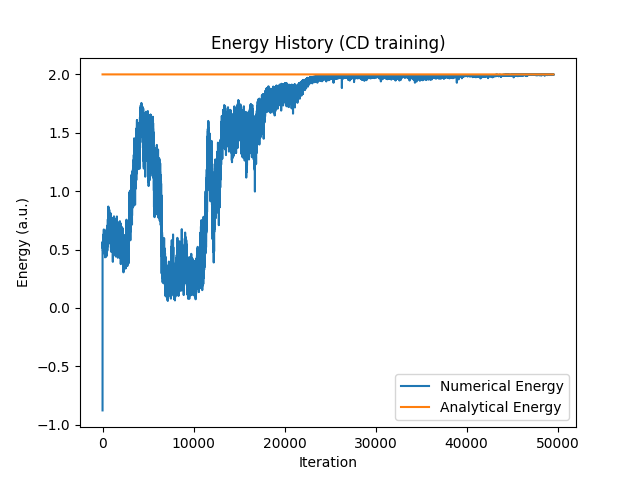
\includegraphics[width=\textwidth,height=0.6\textheight,keepaspectratio]{impoCDnoInteract.png}
    \caption{Energy convergence per iteration for Contrastive Divergence}
    \label{fig:figure2b}
  \end{minipage}
  \hfill
  \begin{minipage}[b]{0.3\textwidth}
    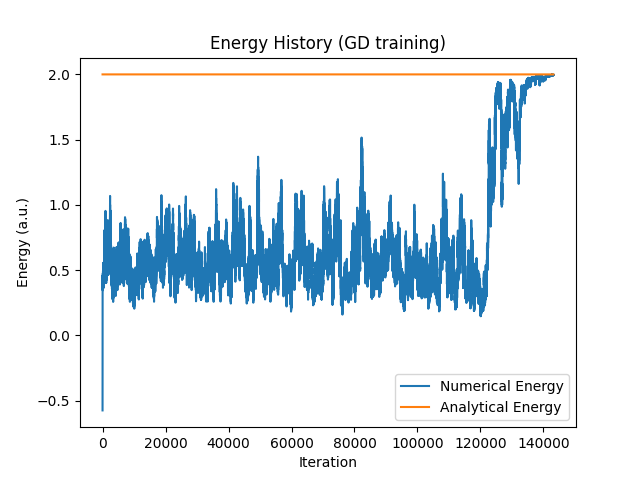
\includegraphics[width=\textwidth,height=0.6\textheight,keepaspectratio]{impoGDnoInteract.png}
    \caption{Energy convergence per iteration for Gradient Descent}
    \label{fig:figure2c}
  \end{minipage}
    \caption*{Here we see how the energy converges over iterations for importance sampling \newline
    $\eta = 0.005$, $h.u. = 16$}

\end{figure}
\newline
Again we see much the same results. The only real difference is that CD more consistently trends towards the analytical value rather than plateauing at another value for a while. \newline
We see a bigger difference in the accompanying table:
\begin{table}[ht!]
    \centering
    \begin{tabular}{c|c|c}
     Type& Result [a.u.]& Error [a.u.]&
     \hline
     PCD&  2.00& 2.51\times10^{-9}\\
     CD& 2.00& 1.50\times10^{-7}\\
     GD& 2.00& 4.38\times10^{-7}
    \end{tabular}
    \caption{The results given importance sampling and a blocking analysis with the following variables:
    \newline MC Cycles: 4992, Hidden Units: 16, Visible Units: 4, $\eta$: 0.005, Sweeps: 100, Chain length: 100
    }
    \label{tab:impo}
\end{table}
\newline
Here we see that generally the errors are improved by a factor of 1/100th, whilst the predicted value remains the same. Again we also see the same order of performance in terms of errors when it comes to the types of training, where PCD vastly outperforms the other methods of training. \newpage
We now wish to examine the interactive case. Sadly, we weren't able to correctly implement this method. Namely, an issue where the particles converge at a single point, thus leading to values approaching infinity in the case of Eq. [\ref{H1}]. This leads to plots like these:
\begin{figure}[ht!]
    \centering
    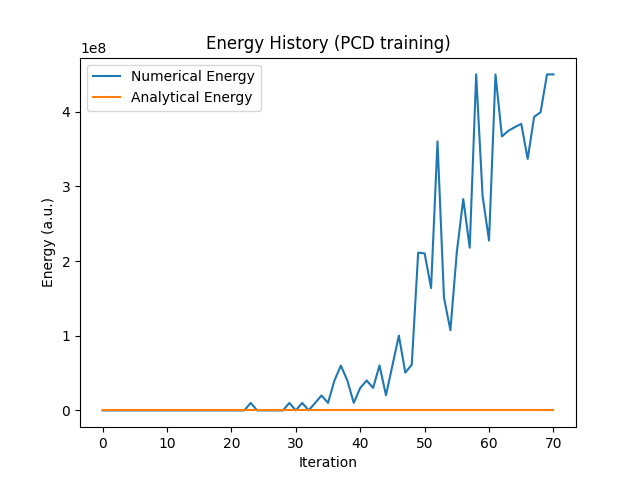
\includegraphics[scale=0.5]{metroPCDInteract.png}
    \caption{The energy grows exponentially as the particles approach the same location, in this case for PCD with Metropolis sampling, but this is true for every other training method and sampler too.}
    \label{figInfinity}
\end{figure}
\newline
which sadly tells us next to nothing.
\section{Discussion}
\subsection{Results and errors}
Firstly, I want to discuss the results. As seen, the results in the case of both metropolis and importance sampling for all methods yield an energy of $2.0$, which is the nominal value. This seems a little too good to be true, and I suspect there's some fishy business with the code. Of course, I ultimately have nothing to base this on, but the code does occasionally produce results in the range of $2.0 \pm 0.10$, which is a little more comforting but still not enough. Generally the code almost always produces an energy value of $2.0$.
\subsection{Code and variable exploration}
We were asked to play around with variables and examine their effect of the code. Generally, atleast according to theory, as we increase most variables we'll see an increase in numerical accuracy (cycles, sweep, chain length, etc.). While many of these variables are straight forward, one that is interesting and unique to the RBM in particular are the hidden units. Typically, in the case of RBMs, the hidden units model the underlying complex relationships and features of the model (in our case the wavefunction). In my case, 16 hidden units was what I used the most, and I found it to be sufficent for numerical accuracy. Another quirk with the hidden units is that, as they increase, the convergence time logarithmically decreases. \newline
Another quirk of the code I feel like is worth pointing out is the variable \texttt{N\textunderscore SCALE}. While you'd think letting the state of the system be of shape $(1,4)$ would be sufficent, this in my case did not work. Introducing then a variable \texttt{N\textunderscore SCALE} such that the state is of shape $(\texttt{N\textunderscore SCALE}, 4)$ and then scaling the energy (which would be \texttt{N\textunderscore SCALE}x higher than nominal value) yielded very good results. The reason for this I could not deduce, I tried letting \texttt{N\textunderscore SCALE} be 1, 10, 50 and 100 respectively and it produced correct results for the latter three.
\subsection{Replacing the RBM with a Neural Network}
One (admittedly optional) part of the project was to see if we can replace the RBM with a Neural Network. While this was optional (and thus left for the end), I wanted to explore it as it is relevant for my Thesis. However, I had trouble getting it work, or rather, how I was supposed to train the Network effectively. Ultimately, I decided upon a very heavy-handed, probably not correct at all solution where it is simply trained based on whether the particles are interactive or not and the analytical energy values. This yielded some results, namely:
\begin{table}[ht!]
    \centering
    \begin{tabular}{c|c|c}
         Interact?& Result [a.u.]& Error [a.u.]  \\
         \hline
         No& 1.99& 1.70\times10^{-8} \\
         Yes& 3.00& 1.5\times10^{-8}
    \end{tabular}
    \caption{The energy estimated by the Neural Network based on whether or not the particles are interactive.}
    \label{tab:my_label}
\end{table}
\newline 
The issue I ran into mainly was that it was hard to train the network in the case of interactive fermions. In the case of non-interacting fermions, it would've been easy as the energy of such a system is known numerically through Eq. [\ref{enrgy}], but this is not the case for the interactive system. Thus it would've been very hard to train the network for anything but the non-interactive case, and ultimately (probably) useless in the case of interaction between the particles.
\section{Conclusion}
In closing, we've used a Restricted Boltzmann Machine to simulate the wave function of a Quantum Mechanical System of Fermions. We've examine how the RBM can be used to accurately predict the local energy of a two fermion system of two degrees of freedom without interaction for several different training and sampling methods. We've also tried to examine the interactive case to less than stellar results. Lastly, we tried our hand using a deep network instead to model the energy, and found that it too was sufficient, albeit with some caveats. \newpage
\bibliographystyle{plainurl}
\bibliography{citations.bib}
\newpage
\renewcommand*\appendixpagename{\Large Appendices}
\appendixpage
\addappheadtotoc
\renewcommand{\thesubsection}{\Alph{subsection}}
\subsection{Expression in 1a)} \label{AppEn}
Given the definition of the Hamiltonian in Eq. [\ref{ham}] and the accompanying local energy in Eq. [\ref{locEn}] we may express the energy:
\begin{equation*}
    E_L = \frac{1}{\Psi} \hat H \Psi
\end{equation*}
as:
\begin{equation*}
    E_L = \frac{1}{\Psi} \left[ \sum_{i=1}^N \left( -\frac{1}{2} \nabla_i^2 + \frac{1}{2} \omega^2 r^2_i \right) + \sum_{i<j} \frac{1}{r_{ij}}\right] \Psi
\end{equation*}
We can rewrite this as:
\begin{equation*}
    E_L = -\frac{1}{2\Psi} \sum_{i=1}^N \sum_{d=1}^D \frac{\delta^2 \Psi}{\delta x_{id}^2} + \frac{1}{2}\omega^2 \sum_{i=1}^N r_i^2 + \sum_{i<j} \frac{1}{r_{ij}}
\end{equation*}
Using then that:
\begin{equation*}
    \frac{1}{\Psi} \frac{\delta^2}{\delta x^2} \Psi = \left(\frac{\delta}{\delta x} \ln \Psi \right)^2 + \frac{\delta^2}{\delta x^2} \ln \Psi
\end{equation*}
we can rewrite this as:
\begin{equation}
    E_L = \frac{1}{2} \sum_{i=1}^N \sum_{d=1}^D \left[-\left(\frac{\delta}{\delta x_{id}} \ln \Psi \right)^2 - \frac{\delta^2}{\delta x_{id}^2} \ln \Psi + \omega^2 x_{id}^2 \right] + \sum_{i<j} \frac{1}{r_{ij}}
\end{equation}
where $N$ is the number of particles and $D$ is the degrees of freedom, as above.
\subsection{Markov Chains} \label{AppMa}
Markov chains are a mathematical framework used to describe a sequence of states or events, where the next state depends only on the current state. Markov chains are incredibly flexible and employed in many fields, able to both model and analyze dynamic processes with random and state dependency.
\newline
Mathematically, we may describe a Markov chain as a series of states ${S_1, S_2, \ldots, S_n}$ and a transition matrix $\mathcal{P}$ where a given element $\mathcal{P}_{ij}$ represents the probability of $S$ transitioning from $S_i$ to $S_j$
\newline
Additionally, the following must hold true
\begin{equation*}
    \sum_{i,j}^N \mathcal{P}_{ij} = 1
\end{equation*}
The idea is that the steady-state (or convergent state) distribution will remain unchanged when multiplied by the transition matrix $\mathcal{P}$, allowing us to converge.
\subsection{Code}
Any code can be found at my \href{https://github.com/simloken/FYS4411/tree/main/Project_2}{github}
\end{document}
